% Source: AESP_466_ClassWork/Assignments/Assignment_3/textbook_example_problems/E5.4/wing_planform_tikz.tex
\documentclass[tikz,border=8pt]{standalone}
\usetikzlibrary{arrows.meta,calc}

% USC Brand Colors
\definecolor{USCGarnet}{HTML}{73000A}
\definecolor{USCAtlantic}{HTML}{466A9F}
\definecolor{USCBlack}{HTML}{000000}

\begin{document}
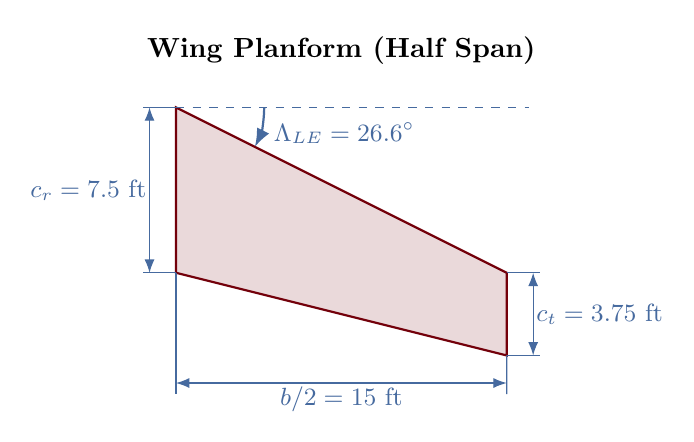
\begin{tikzpicture}[>=Latex,line cap=butt,line join=miter]

% Scale: 1 unit = 1 ft, then scale down for display
\def\scale{0.28}

% Wing geometry
\def\rootchord{7.5}
\def\tipchord{3.75}
\def\semispan{15}
\def\tipoffset{7.5}  % LE sweep offset (tan(26.6°) * 15 = 7.5)

% Standard aerospace convention:
% y-axis: spanwise (horizontal, pointing right)
% x-axis: chordwise/aft (vertical, pointing down)

\begin{scope}[scale=\scale]

% Wing coordinates (y = spanwise, x = chordwise)
% In TikZ: first coord is horizontal (y), second is vertical (x, but inverted so down is positive)
\coordinate (RootLE) at (0,0);
\coordinate (RootTE) at (0,-\rootchord);
\coordinate (TipLE) at (\semispan,-\tipoffset);
\coordinate (TipTE) at (\semispan,-\tipoffset-\tipchord);

% Fill wing
\fill[USCGarnet!15] (RootLE) -- (TipLE) -- (TipTE) -- (RootTE) -- cycle;

% Wing outline
\draw[USCGarnet,thick] (RootLE) -- (TipLE) -- (TipTE) -- (RootTE) -- cycle;


% ---- DIMENSIONS ----

% Root chord dimension (left side)
\draw[USCAtlantic,thin] (RootLE) -- ++(-1.5,0);
\draw[USCAtlantic,thin] (RootTE) -- ++(-1.5,0);
\draw[<->,USCAtlantic] (-1.2,0) -- (-1.2,-\rootchord)
    node[midway,left,fill=white,inner sep=1pt,font=\small] {$c_r = 7.5$ ft};

% Tip chord dimension (right side)
\draw[USCAtlantic,thin] (TipLE) -- ++(1.5,0);
\draw[USCAtlantic,thin] (TipTE) -- ++(1.5,0);
\draw[<->,USCAtlantic] (\semispan+1.2,-\tipoffset) -- (\semispan+1.2,-\tipoffset-\tipchord)
    node[midway,right,fill=white,inner sep=1pt,font=\small] {$c_t = 3.75$ ft};

% Semispan dimension (bottom)
\draw[USCAtlantic,thin] (RootTE) -- (0,-\rootchord-5.5);
\draw[USCAtlantic,thin] (TipTE) -- (\semispan,-\rootchord-5.5);
\draw[<->,USCAtlantic] (0,-\rootchord-5) -- (\semispan,-\rootchord-5)
    node[midway,below,fill=white,inner sep=1pt,font=\small] {$b/2 = 15$ ft};

% ---- SWEEP ANGLE ----
% Reference line (spanwise direction from root LE)
\draw[USCAtlantic,dashed,thin] (RootLE) -- (\semispan+1,0);

% Sweep angle arc (manual arc for control)
\draw[USCAtlantic,thick,->] (4,0) arc[start angle=0, end angle=-26.6, radius=4]
    node[pos=0.5,right,xshift=3pt,yshift=-2pt,fill=white,inner sep=1pt,font=\small] {$\Lambda_{LE} = 26.6^\circ$};

% Title
\node[above,font=\bfseries] at (\semispan/2,1.5) {Wing Planform (Half Span)};

\end{scope}

\end{tikzpicture}
\end{document}
